\documentclass[11pt]{article}
\usepackage[utf8]{inputenc}
\usepackage[T1]{fontenc}
\usepackage{lmodern}
\usepackage[margin=1in]{geometry}
\usepackage{amsmath,amssymb,amsthm,mathtools}
\usepackage{booktabs}
\usepackage{enumitem}
\usepackage{graphicx}
\usepackage{microtype}
\usepackage{pgfplots}
\pgfplotsset{compat=1.17}
\usepackage[colorlinks=true,linkcolor=blue,citecolor=blue,urlcolor=blue]{hyperref}
\hypersetup{pdftitle={An explicit Bellman function for disjoint partitions: the sharp logarithmic gain for three families},
  pdfauthor={Paata Ivanisvili}}

\newtheorem{theorem}{Theorem}[section]
\newtheorem{lemma}{Lemma}[section]
\newtheorem{proposition}[lemma]{Proposition}
\newtheorem{corollary}[lemma]{Corollary}
\theoremstyle{definition}
\newtheorem{remark}[lemma]{Remark}
\numberwithin{equation}{section}

\newcommand{\one}{\mathbf 1}
\newcommand{\R}{\mathbb R}
\newcommand{\ip}[2]{\langle #1,#2\rangle}
\newcommand{\KLb}[2]{d(#1\,\|\,#2)}
\newcommand{\KL}[2]{D(#1\,\|\,#2)}
\newcommand{\Azero}{2000}
\newcommand{\cA}{\mathcal A}
\newcommand{\cF}{\mathcal F}
\newcommand{\Var}{\operatorname{Var}}
\newcommand{\Cov}{\operatorname{Cov}}
\newcommand{\osc}{\operatorname{osc}}
\newcommand{\dlo}{\underline d}
\newcommand{\dhi}{\overline d}
\newcommand{\Smin}{S_{\min}}
\newcommand{\bmin}{b_{\min}}

\title{An explicit Bellman function for disjoint partitions:\\ the sharp logarithmic gain for three families}
\author{Paata Ivanisvili\\[4pt]
{\small Department of Mathematics, University of California, Irvine}\\
{\small\href{mailto:pivanisv@uci.edu}{\texttt{pivanisv@uci.edu}}}}
\date{}

% --- AI disclosure (site) ---
\usepackage{etoolbox}
\makeatletter
\patchcmd{\@maketitle}{\null}{\null\par{\centering\small\itshape
This proof was generated on September 23, 2026, by Grok Bot using Cursor’s agents, guided by several prompts from Paata Ivanisvili
\par}\vskip 1.2em}{}{}
\makeatother
% --- end AI disclosure ---
\begin{document}
\maketitle

\begin{abstract}
For families $\cF_1,\cF_2,\cF_3$ of subsets of $[m]=\{1,\dots,m\}$ let $N(\cF_1,\cF_2,\cF_3)$ be the number of ordered
partitions $[m]=T_1\sqcup T_2\sqcup T_3$ with $T_j\in\cF_j$. Every function $B\ge0$ on $[1,\infty)^3$ with $B(1,1,1)\ge1$ that
satisfies $B(x_0+x_1,y_0+y_1,z_0+z_1)\ge B(x_1,y_0,z_0)+B(x_0,y_1,z_0)+B(x_0,y_0,z_1)$ for all $x_i,y_i,z_i\ge0$ (with $B:=0$
when an argument is less than $1$), a \emph{Bellman function}, gives $N\le B(|\cF_1|,|\cF_2|,|\cF_3|)$. The classical choice $B=(xyz)^c$,
$c=\ln3/\ln(27/4)$, yields the Kane--Tao bound $N_3(X)\le|X|^{3c}$ for the number $N_3(X)$ of ordered pairs of disjoint
members of a family $X$ whose union also belongs to $X$. We give an explicit closed-form Bellman function that captures the
sharp logarithmic gain,
\[
B(x,y,z)=(xyz)^c\Bigl(\frac GM\Bigr)^{\kappa}\Bigl(1+\frac{\ln(xyz)}{2000}\Bigr)^{-\gamma},
\]
where $G$ is the geometric mean of $x,y,z$, $M$ is their power mean of order $\alpha/\ln(xyz)$,
$\gamma=\ln(27/16)/(2\ln(27/4))$, and $\alpha,\kappa$ are explicit constants built from $\ln2$ and $\ln3$.
Consequently $N_3(X)\le2.44\,|X|^{3c}(1+\ln|X|)^{-\gamma}$, and the exponent $\gamma$ is sharp. The proof combines the Gibbs
variational principle with an exact decomposition of the slack; finitely many explicit numerical inequalities are verified
rigorously in interval arithmetic. High-precision numerical tests confirm the result and indicate that the shift $2000$ can
be lowered to about $29$.

\medskip
\noindent\textbf{Keywords:} Bellman function, disjoint partitions, Kane--Tao bound, logarithmic gain, power mean, entropy,
computer-assisted proof.

\noindent\textbf{2020 Mathematics Subject Classification:} 05D05; 05A20, 39B62, 65G30, 94A17.
\end{abstract}

%======================================================================
\section{Introduction}\label{sec:intro}
%======================================================================
For finite families $\cF_1,\cF_2,\cF_3$ of subsets of $[m]$ let $N(\cF_1,\cF_2,\cF_3)$ be the number of triples
$(T_1,T_2,T_3)\in\cF_1\times\cF_2\times\cF_3$ with $T_1\sqcup T_2\sqcup T_3=[m]$, and for a family $X$ of subsets of $[m]$ let
$N_3(X)$ be the number of triples $(T_1,T_2,T)\in X^3$ with $T=T_1\sqcup T_2$; thus $N_3(X)=N(X,X,X^c)$ with
$X^c=\{[m]\setminus T:T\in X\}$. Kane and Tao~\cite{KT17} proved
\[
N_3(X)\le|X|^{c(3)},\qquad c(3)=\frac{\ln27}{\ln(27/4)}=1.72598\ldots,
\]
with a sharp exponent, and the bound was extended to partitions into any number of parts in~\cite{Iva17}. Whether a power of
$\ln|X|$ can be gained was asked in the discussion of~\cite{Tao17}. The companion paper~\cite{P} proves the sharp refinement
$N_3(X)\le C_3|X|^{c(3)}(1+\ln|X|)^{-\gamma_3}$ with $\gamma_3=\frac{2-c(3)}2=0.13700\ldots$ and $C_3\le359$, together with its
analogue for any number of parts; its Bellman function has the form $V_0\min\{1,\Theta\}$, with an envelope $V_0$ of weighted
bounds and an explicit correction $\Theta$. In this paper we show that for three parts a single closed-form Bellman function
gives the sharp bound, with the constant $2.44$ in place of $C_3$.

\paragraph{The main inequality.}
Sorting the partitions according to the part that contains the element $m$ leads to the following inequality for a function
$B\colon[1,\infty)^3\to[0,\infty)$, extended by $B(x,y,z):=0$ if $\min\{x,y,z\}<1$: for all $x_0,x_1,y_0,y_1,z_0,z_1\ge0$,
\begin{equation}\label{eq:main}
B(x_0+x_1,\,y_0+y_1,\,z_0+z_1)\ \ge\ B(x_1,y_0,z_0)+B(x_0,y_1,z_0)+B(x_0,y_0,z_1).
\end{equation}
We call~\eqref{eq:main} the \emph{main inequality}, and a function that satisfies it and $B(1,1,1)\ge1$ a \emph{Bellman
function}. Every Bellman function bounds the number of partitions (Lemma~\ref{lem:count}):
\begin{equation}\label{eq:count}
N(\cF_1,\cF_2,\cF_3)\le B(|\cF_1|,|\cF_2|,|\cF_3|),\qquad\text{in particular}\qquad N_3(X)\le B(|X|,|X|,|X|).
\end{equation}

\paragraph{The classical Bellman function.}
The function
\begin{equation}\label{eq:classical}
B(x,y,z)=(xyz)^{c},\qquad c=\frac{c(3)}3=\frac{\ln3}{\ln(27/4)}=0.57532\ldots,
\end{equation}
satisfies the main inequality~\cite{KT17,Iva17} (it is also the case $\pi=U$ of Remark~\ref{rem:envelope}), and
$B(x,x,x)=x^{c(3)}$; by~\eqref{eq:count} this gives the Kane--Tao bound.

\paragraph{The new Bellman function.}
Let $\lambda=\ln2$, $\mu=\ln\frac{27}4$, and
\begin{equation}\label{eq:const}
\begin{gathered}
\gamma=\frac{\ln(27/16)}{2\ln(27/4)}=0.13700\ldots,\\[2pt]
\alpha=\frac{3\mu}{2\lambda}\Bigl(\frac9\lambda-1-\frac1\gamma\Bigr)=19.3618\ldots,\qquad
\kappa=\frac{9\gamma\mu}{\lambda^2\alpha}=0.25311\ldots;
\end{gathered}
\end{equation}
note that $\gamma=\frac{2-3c}2=\gamma_3$. For $x,y,z\ge1$ let
\[
G=(xyz)^{1/3},\qquad M=\Bigl(\frac{x^t+y^t+z^t}3\Bigr)^{1/t},\qquad t=\frac\alpha{\ln(xyz)}
\]
be the geometric mean and the power mean of order $t$ (with $G/M:=1$ at $x=y=z=1$), and put
\begin{equation}\label{eq:newB}
\boxed{\;B(x,y,z)=(xyz)^{c}\,\Bigl(\frac GM\Bigr)^{\kappa}\,\Bigl(1+\frac{\ln(xyz)}{2000}\Bigr)^{-\gamma}\;}
\end{equation}
More generally, for $0<A\le\infty$ let $B_A$ be defined by~\eqref{eq:newB} with $2000$ replaced by $A$; thus $B=B_{2000}$, and
$B_\infty=(xyz)^c(G/M)^\kappa$. On the diagonal $G=M$, so
\begin{equation}\label{eq:diag}
B(x,x,x)=\frac{x^{3c}}{\bigl(1+\frac3{2000}\ln x\bigr)^{\gamma}}\ \le\ 2.44\,\frac{x^{3c}}{(1+\ln x)^{\gamma}},
\end{equation}
because $1+\frac3{2000}\ln x\ge\frac3{2000}(1+\ln x)$ and $(2000/3)^\gamma=2.4373\ldots$.

\begin{theorem}\label{thm:main}
For every $A\in[\Azero,\infty]$ the function $B_A$ satisfies the main inequality~\eqref{eq:main}, and $B_A(1,1,1)=1$.
Consequently, for all finite families $\cF_1,\cF_2,\cF_3$ and all nonempty finite families $X$ of subsets of $[m]$,
\[
N(\cF_1,\cF_2,\cF_3)\le B_A(|\cF_1|,|\cF_2|,|\cF_3|)\qquad\text{and}\qquad
N_3(X)\le\frac{|X|^{3c}}{\bigl(1+\frac3A\ln|X|\bigr)^{\gamma}}\le\Bigl(\frac A3\Bigr)^{\gamma}\frac{|X|^{3c}}{(1+\ln|X|)^{\gamma}} .
\]
In particular~\eqref{eq:newB} is a Bellman function, and $N_3(X)\le2.44\,|X|^{c(3)}(1+\ln|X|)^{-\gamma_3}$.
\end{theorem}

The exponent $\gamma_3$ is sharp: for the two-layer families $X_m=\{T\subseteq[m]:|T|\in\{\frac m3,\frac{2m}3\}\}$ one has
$N_3(X_m)\asymp|X_m|^{c(3)}(\ln|X_m|)^{-\gamma_3}$~\cite[Thm.~1.1(b)]{P}. Off the diagonal $G<M$ by the power-mean inequality,
so already $B_\infty=(xyz)^c(G/M)^\kappa$ improves on the classical function~\eqref{eq:classical}, and the logarithmic factor
gains the extra $(\ln x)^{-\gamma}$ on the diagonal. The constants $\alpha$ and $\kappa$ are forced by the behaviour of the main
inequality near the balanced configuration (Section~\ref{sec:why}). The shift $2000$ comes from the explicit constants of the
proof and is far from optimal: numerically (Section~\ref{sec:num}), $B_A$ satisfies the main inequality if and only if
$A\ge A_*\approx29.05$, the binding sizes being $\ln(xyz)\approx40$. With $A=A_*$ the diagonal constant would be
$(A_*/3)^\gamma\approx1.365$ (for $A=30$ it is $10^\gamma=1.371$).

\paragraph{Outline.} Section~\ref{sec:bellman} derives the counting bound~\eqref{eq:count} from the main inequality, explains
the choice of the constants in logarithmic coordinates, and outlines the proof of Theorem~\ref{thm:main}.
Section~\ref{sec:num} reports high-precision numerical tests. The proof is given in Appendix~\ref{app:proof}, and the
computer-assisted steps, together with the scripts that perform them, are described in Appendix~\ref{app:cap}.

%======================================================================
\section{The Bellman function}\label{sec:bellman}
%======================================================================
\subsection{From the main inequality to the counting bound}

\begin{lemma}\label{lem:count}
Let $B\colon[1,\infty)^3\to[0,\infty)$, extended by $0$ as in Section~\ref{sec:intro}, satisfy the main inequality and
$B(1,1,1)\ge1$. Then~\eqref{eq:count} holds for all $m\ge0$, all families $\cF_1,\cF_2,\cF_3$ and all families $X$ of subsets
of $[m]$.
\end{lemma}
\begin{proof}
We use induction on $m$. For $m=0$ the only subset of $[m]$ is $\emptyset$, so $N(\cF_1,\cF_2,\cF_3)=1\le B(1,1,1)$ if
$\cF_1=\cF_2=\cF_3=\{\emptyset\}$, and $N(\cF_1,\cF_2,\cF_3)=0$ otherwise. Let $m\ge1$. Sorting the partitions by the part that
contains $m$ gives $N(\cF)=N(\cF^{(1)})+N(\cF^{(2)})+N(\cF^{(3)})$, where $\cF^{(i)}$ consists of the sets of $\cF_i$ that contain
$m$ (with $m$ removed) and the sets of $\cF_j$, $j\ne i$, that do not; these are families of subsets of $[m-1]$. If
$x_1,y_1,z_1$ are the numbers of sets in $\cF_1,\cF_2,\cF_3$ that contain $m$ and $x_0,y_0,z_0$ the numbers of the other sets,
then the triples $\cF^{(1)},\cF^{(2)},\cF^{(3)}$ have sizes $(x_1,y_0,z_0)$, $(x_0,y_1,z_0)$, $(x_0,y_0,z_1)$. By the induction
hypothesis and the main inequality,
\begin{align*}
N(\cF)&\le B(x_1,y_0,z_0)+B(x_0,y_1,z_0)+B(x_0,y_0,z_1)\\
&\le B(x_0+x_1,\,y_0+y_1,\,z_0+z_1)=B(|\cF_1|,|\cF_2|,|\cF_3|).
\end{align*}
Finally $N_3(X)=N(X,X,X^c)$ and $|X^c|=|X|$.
\end{proof}

\subsection{Logarithmic coordinates and the choice of the constants}\label{sec:why}
Throughout, $\lambda=\ln2$, $\mu=\ln\frac{27}4$, $\nu=\ln\frac{27}{16}$, and $c,\gamma,\alpha,\kappa$ are the constants
of~\eqref{eq:classical} and~\eqref{eq:const}; thus $3c=c(3)$ and $\gamma=\frac\nu{2\mu}=\frac{2-3c}2=\gamma_3$. In logarithmic
coordinates $\ell=(\ln x,\ln y,\ln z)$, $s=\ell_1+\ell_2+\ell_3$,
\begin{gather*}
\ln B_A=F(\ell)-\gamma\ln\Bigl(1+\frac sA\Bigr),\qquad F(\ell)=c\,s-K\,s\,L\Bigl(\frac\ell s\Bigr),\\
L(w)=\ln\Bigl(\frac13\sum_{j=1}^3e^{\alpha(w_j-\frac13)}\Bigr),\qquad K=\frac\kappa\alpha ,
\end{gather*}
because $\ln M=\frac s\alpha\ln\bigl(\frac13\sum_je^{\alpha\ell_j/s}\bigr)$ and $\ln G=\frac s3$. The function $e^F$ is the lower
envelope of an explicit family of weighted bounds $\prod_j|\cF_j|^{b_j(\pi)}$, $\pi\in\Delta$, each of which satisfies the
main inequality (Lemma~\ref{lem:F} and Remark~\ref{rem:envelope}); this plays the role of $V_0$ in~\cite{P}, and the single factor
$(1+s/A)^{-\gamma}$ plays the role of $\min\{1,\Theta\}$. Near the diagonal,
$K\,L(\frac13\one+y)=\beta|y|^2+\kappa_3\,y_1y_2y_3+O(|y|^4)$ with $\beta=\frac{K\alpha^2}6$ and $\kappa_3=\frac{K\alpha^3}6$, and
both numbers are forced. (i) Per step, the logarithmic factor loses $\gamma\mu/s$ to leading order, and the curvature of the
profile gains $\frac23\beta\lambda^2/s$; the two balance exactly for $\beta=\frac{3\nu}{4\lambda^2}=0.8168\ldots$ (a larger
$\beta$ destroys admissibility, a smaller one loses at order $1/s$). (ii) The entropic (``layer'') profile has the cubic term
$\kappa_3=\frac{3\mu^2}{\lambda^3}\bigl(\frac{27\gamma}{4\lambda}-\frac{3(1+\gamma)}4\bigr)=15.81\ldots$, and admissibility forces
the profile to match it (otherwise the admissibility gap $Q$ of Proposition~\ref{prop:Q} changes sign at the balanced point).
The log-sum-exp profile is the simplest one with independent quadratic and cubic coefficients; matching $\beta$ and $\kappa_3$
gives $\alpha=\kappa_3/\beta$ and $\kappa=6\beta/\alpha$, i.e.\ the values~\eqref{eq:const}. The only remaining freedom is the
shift $A$ in the logarithmic factor, which absorbs the errors of order $s^{-2}$.

\subsection{Structure of the proof}\label{sec:structure}
The proof is given in Appendix~\ref{app:proof}. By the Gibbs variational principle the main inequality is
equivalent to the nonnegativity of an explicit slack $E(\ell,u,q)$, where $u\in[0,1]^3$ are the split fractions and $q$ is a
probability vector on the three children (Lemma~\ref{lem:red}); $E$ is increasing in $A$, so $A=\Azero$ suffices. Two exact
identities do most of the work: the envelope representation of $F$ (Lemma~\ref{lem:F}) and a decomposition of $E$ into five
explicit terms (Lemma~\ref{lem:slack}). Four of them are nonnegative as soon as the \emph{admissibility gap}
$Q(q)=\frac{I(q)}{S(q)}-K\,L\bigl(\frac{h(q)}{S(q)}\bigr)$ is nonnegative (Proposition~\ref{prop:Q}); the fifth is the loss
caused by the logarithmic factor. Away from the balanced configuration the gap, a Kullback--Leibler term in the split, or a
Kullback--Leibler term in the shape absorbs the loss (Proposition~\ref{prop:far}). Near it, a second-order expansion with explicit
constants reduces everything to an inequality in the single variable $s$ (Proposition~\ref{prop:near}). The finitely many
numerical facts used are verified rigorously in ball arithmetic, or exactly in symbolic arithmetic (Appendix~\ref{app:cap}).

%======================================================================
\section{Numerical verification}\label{sec:num}
%======================================================================
For the main inequality we write $\delta=\ln\mathrm{LHS}-\ln\mathrm{RHS}$ (so the relative slack is
$1-\mathrm{RHS}/\mathrm{LHS}=1-e^{-\delta}$; $\delta=+\infty$ if the right side is $0$), parametrised by the parent sizes
$X=e^{\ell_1}$, $Y=e^{\ell_2}$, $Z=e^{\ell_3}$ and the split fractions $u=(x_1/X,y_1/Y,z_1/Z)$. Equality holds at the
\emph{trivial splits} $u\in\{e_1,e_2,e_3\}$ (e.g.\ $x_0=y_1=z_1=0$), where a single child survives and equals the parent;
it was not observed anywhere else. As $u$
approaches a trivial split the slack vanishes linearly, and near the balanced configuration it is of order $s^{-2}$; the worst-case
slack is therefore reported in these normalisations. All values are computed with \texttt{mpmath} at 50 significant digits from
the logarithmic form of Section~\ref{sec:why} (the closed form~\eqref{eq:newB} agrees with it to a relative error of
$5\cdot10^{-50}$ at 300 random points). Script: \texttt{verification/numerics.py} (6.5 minutes on 8 cores); raw output:
\texttt{verification/results/}.

\paragraph{Integer grid.} All integer parents $1\le X,Y,Z\le24$ and all splits $0\le x_1\le X$, $0\le y_1\le Y$, $0\le z_1\le Z$:
$34\,012\,224$ configurations for each $A$, of which $41\,472$ are trivial splits (where $|\delta|<10^{-25}$ was checked) and
$546\,048$ have a vanishing right side.

\begin{center}
\begin{tabular}{lccc}
\toprule
$A$ & $\min\delta$ (non-trivial splits) & relative slack $1-e^{-\delta}$ & attained at $(x_1,x_0,y_1,y_0,z_1,z_0)$\\
\midrule
$2000$ & $7.1444\cdot10^{-3}$ & $0.71\%$ & $(1,4,1,4,14,9)$\\
$30$ & $7.6306\cdot10^{-4}$ & $0.076\%$ & $(1,4,1,4,12,8)$\\
$\infty$ & $7.2582\cdot10^{-3}$ & $0.72\%$ & $(1,4,1,4,14,9)$\\
\bottomrule
\end{tabular}
\end{center}

\paragraph{Random samples.} $400\,000$ real configurations per class and per value of $A$ (seeded; the same samples for each
$A$), in five classes: \emph{generic} ($s=10^{U(-3,5)}$, shape $\ell/s$ uniform on the simplex, $u$ uniform in $[0,1]^3$);
\emph{balanced} ($s=10^{U(0,6)}$, shape within $\approx s^{-1/2}$ of $\frac13\one$, $u_j=\frac13+N(0,\sigma^2)$,
$\sigma=10^{U(-4,-0.7)}$); \emph{faces} (one or two parent sizes in $[1,1.1]$ or exactly $1$, and $u_j\in\{\varepsilon,1-\varepsilon,
U(0,1)\}$, $\varepsilon=10^{U(-12,-1)}$); \emph{near-trivial} ($u=e_k+O(10^{U(-10,-0.5)})$); \emph{child at threshold}
(an active child one of whose sizes is $e^{\varepsilon}$, $\varepsilon=10^{U(-12,-1)}$, i.e.\ just above the jump of $B$ from $0$
to $\ge1$). The table gives the number of samples with a positive right side (for the others the inequality is trivial), and the
minima of $\delta$ and of the normalised slack appropriate to the class: $s^2\delta$ (over the samples with $s\ge10$), or
$\delta/\operatorname{dist}(u)$ with $\operatorname{dist}(u)=\min_k|u-e_k|_1$.

\begin{center}
\begin{tabular}{lrlccc}
\toprule
class & RHS${}>0$ & minimum of & $A=2000$ & $A=30$ & $A=\infty$\\
\midrule
generic & $214\,515$ & $\delta$ & $1.02\cdot10^{-3}$ & $4.92\cdot10^{-4}$ & $1.13\cdot10^{-3}$\\
 & & $s^2\delta$ & $0.976$ & $0.258$ & $0.990$\\[2pt]
balanced & $368\,294$ & $\delta$ & $2.33\cdot10^{-9}$ & $6.36\cdot10^{-10}$ & $2.69\cdot10^{-7}$\\
 & & $s^2\delta$ & $0.981$ & $0.181$ & $0.994$\\[2pt]
faces & $68\,463$ & $\delta$ & $2.46\cdot10^{-12}$ & $2.44\cdot10^{-12}$ & $2.46\cdot10^{-12}$\\
 & & $\delta/\operatorname{dist}(u)$ & $0.0100$ & $0.0086$ & $0.0101$\\[2pt]
near-trivial & $384\,027$ & $\delta$ & $1.64\cdot10^{-10}$ & $1.64\cdot10^{-10}$ & $1.64\cdot10^{-10}$\\
 & & $\delta/\operatorname{dist}(u)$ & $0.0219$ & $0.0167$ & $0.0221$\\[2pt]
child at threshold & $399\,707$ & $\delta$ & $6.64\cdot10^{-4}$ & $6.62\cdot10^{-4}$ & $6.64\cdot10^{-4}$\\
 & & $s^2\delta$ & $1.036$ & $0.425$ & $1.048$\\
\bottomrule
\end{tabular}
\end{center}

\paragraph{Worst case at fixed size.} For each $s$ the minimum of $s^2\delta$ over the shape $\ell/s$ and over
$u\in[0.02,0.98]^3$ (the near-trivial region is covered by the samples above) was searched by Nelder--Mead from 16 starting
points, with every evaluation in 50-digit arithmetic. Negative entries are violations.

\begin{center}
\begin{tabular}{lrrrrrrrr}
\toprule
$A\ \backslash\ s$ & $10$ & $30$ & $10^2$ & $300$ & $10^3$ & $10^4$ & $10^5$ & $10^6$\\
\midrule
$2000$ & $0.687$ & $3.779$ & $18.89$ & $61.57$ & $167.8$ & $429.8$ & $506.9$ & $516.2$\\
$30$ & $0.105$ & $0.076$ & $0.309$ & $0.857$ & $1.326$ & $1.695$ & $1.795$ & $1.824$\\
$25$ & $0.012$ & $-0.278$ & $-0.489$ & $-0.237$ & $0.089$ & $0.394$ & $0.487$ & $0.515$\\
$22$ & $-0.058$ & $-0.523$ & $-1.000$ & $-0.909$ & $-0.659$ & $-0.387$ & $-0.297$ & $-0.269$\\
\bottomrule
\end{tabular}
\end{center}
For large $s$ the minimal $s^2\delta$ approaches $\gamma\mu\,(A-A_\infty)$ with $\gamma\mu=\frac\nu2=0.2616$ and $A_\infty\approx23.0$
(interpolating linearly between the rows $A=22$ and $A=25$, the zero crossings in $A$ at $s=10^4,10^5,10^6$ are $23.49$, $23.14$,
$23.03$; the direct computation below gives $A_*(10^4)=23.486$); for $A=2000$ this is $\approx517$.

\paragraph{The smallest admissible shift.} For fixed $(s,\ell/s,u)$ the slack is non-decreasing in $A$ (Lemma~\ref{lem:red}), so
it changes sign at a critical value $A_0(s,\ell/s,u)$, and $B_A$ satisfies the main inequality iff $A\ge A_*(s)$ for every $s$,
where $A_*(s)$ is the supremum of $A_0$ over the shape and the split. The curve $A_*(s)$ was computed by maximising $A_0$ (root-finding in $A$; $20\,000$ random seeds and 24 Nelder--Mead
runs per size; \texttt{verification/threshold.py}); at every maximiser the sign change of $\delta$ between $A_0-0.01$ and
$A_0+0.01$ was confirmed in 50-digit arithmetic. The maximum is $A_*=29.05$, attained at $s\approx40$ (Figure~\ref{fig:thr}).

\begin{figure}[ht]
\centering
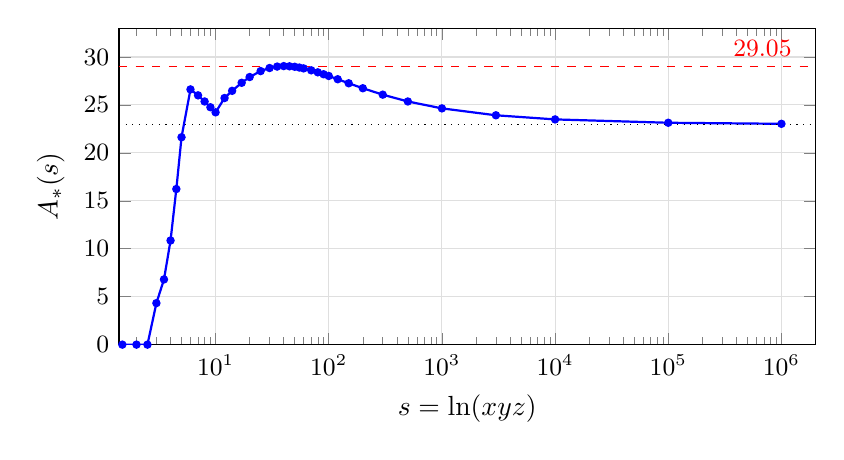
\begin{tikzpicture}
\begin{semilogxaxis}[width=0.86\linewidth,height=5.6cm,xlabel={$s=\ln(xyz)$},ylabel={$A_*(s)$},
  xmin=1.4,xmax=2e6,ymin=0,ymax=33,grid=major,grid style={gray!25},
  ytick={0,5,10,15,20,25,30},tick label style={font=\small}]
\addplot[thick,blue,mark=*,mark size=1.1pt] coordinates {
(1.5,0) (2,0) (2.5,0) (3,4.33) (3.5,6.80) (4,10.86) (4.5,16.23) (5,21.63) (6,26.62) (7,26.00) (8,25.36) (9,24.76)
(10,24.23) (12,25.72) (14,26.47) (17,27.31) (20,27.91) (25,28.53) (30,28.85) (35,29.00) (40,29.05) (45,29.03) (50,28.98)
(55,28.90) (60,28.81) (70,28.61) (80,28.40) (90,28.20) (100,28.02) (120,27.68) (150,27.26) (200,26.74) (300,26.07)
(500,25.36) (1000,24.64) (3000,23.92) (10000,23.49) (100000,23.14) (1000000,23.03)};
\addplot[dashed,red,domain=1.4:2e6,samples=2] {29.05};
\addplot[dotted,black,domain=1.4:2e6,samples=2] {22.94};
\node[red,anchor=south east,font=\small] at (axis cs:1.5e6,29.05) {$29.05$};
\end{semilogxaxis}
\end{tikzpicture}
\caption{The smallest admissible shift $A_*(s)$ at each size $s$. Dashed: its maximum $29.05$; dotted: the large-$s$ limit
$\approx23$. The two rightmost points are the zero crossings in $A$ of the worst-case values in the table above (linear
interpolation between $A=22$ and $A=25$); the others are computed directly.}\label{fig:thr}
\end{figure}

\paragraph{Summary.} No violation was found for $A=2000$, $A=30$ or $A=\infty$: $3.4\cdot10^7$ integer configurations and
$2\cdot10^6$ random real configurations, each evaluated for the three values of $A$, including parents on the faces of
$[1,\infty)^3$, splits near the trivial ones, and children at the activation threshold. For $A=2000$ the worst-case slack is: $\delta\ge7.14\cdot10^{-3}$ (relative slack $0.71\%$)
on the integer grid; $\min s^2\delta=0.687$ at $s=10$, increasing with $s$ to $516$ at $s=10^6$ (asymptotically $\approx517$);
and $\delta\ge0.0100\,\operatorname{dist}(u)$ near the trivial splits. In the proof itself the final one-variable inequality
holds with ratio deficit/gain at most $0.644$ (Appendix~\ref{app:cap}).

\appendix
%======================================================================
\section{\texorpdfstring{Proof of Theorem~\ref{thm:main}}{Proof of the theorem}}\label{app:proof}
%======================================================================
\subsection{Notation and reduction}\label{sec:red}
Let $\Delta=\{q\in[0,1]^3:\sum_jq_j=1\}$, $U=\frac13\one$, $e_1,e_2,e_3$ the unit vectors (the vertices of $\Delta$),
$\one^\perp=\{v\in\R^3:\sum_jv_j=0\}$, $|\cdot|$ the Euclidean norm, and $P$ the orthogonal projection onto $\one^\perp$. We use
$0\ln0=0$,
\begin{gather*}
h(t)=-t\ln t-(1-t)\ln(1-t),\qquad H(q)=-\sum_jq_j\ln q_j,\\
\KLb xy=x\ln\frac xy+(1-x)\ln\frac{1-x}{1-y},\qquad \KL p{p'}=\sum_jp_j\ln\frac{p_j}{p'_j},
\end{gather*}
apply $h$ and $d$ coordinatewise ($h(q)=(h(q_j))_j$, $\KLb qu=(\KLb{q_j}{u_j})_j$), and put $S(q)=\sum_jh(q_j)$. For $p\in\Delta$ and
$f,g\in\R^3$ (functions on $\{1,2,3\}$), $\mathbb E_pf=\sum_jp_jf_j$, $\tilde f=f-\mathbb E_pf$, $\Cov_p(f,g)=\mathbb E_p\tilde f\tilde g$,
$\Var_p(f)=\Cov_p(f,f)$, and $\osc f=\max_jf_j-\min_jf_j$. For $\zeta\in\R^3$ let $\pi(\zeta)=\bigl(e^{\alpha\zeta_j}/\sum_ke^{\alpha\zeta_k}\bigr)_j$.
For $u\in[0,1]^3$ and $i\in\{1,2,3\}$ let $D^{(i)}(u)\in[-\infty,0]^3$,
\[
D^{(i)}_i(u)=\ln u_i,\qquad D^{(i)}_j(u)=\ln(1-u_j)\ (j\ne i),\qquad d_i(u)=-\textstyle\sum_jD^{(i)}_j(u)\in[0,\infty].
\]
For $\ell\in[0,\infty)^3$ let $s=\ell_1+\ell_2+\ell_3$, $\xi=\ell/s\in\Delta$ (if $s>0$), $\ell^{(i)}=\ell+D^{(i)}(u)$ (the children),
$s_i=s-d_i(u)\le s$, $\cA(\ell,u)=\{i:\ell^{(i)}\in[0,\infty)^3\}$ (the active children), and $\Delta(\cA)=\{q\in\Delta:q_i=0\text{ for }i\notin\cA\}$.
Finally $K=\kappa/\alpha$, $\bmin=c-\frac23\kappa=0.40658\ldots$,
\begin{gather*}
L(w)=\ln\Bigl(\frac13\sum_je^{\alpha(w_j-\frac13)}\Bigr),\qquad F(\ell)=cs-Ks\,L(\xi)\ \ (s>0),\qquad F(0)=0,\\
\Phi_A(\ell)=F(\ell)-\gamma\ln\Bigl(1+\frac sA\Bigr),
\end{gather*}
so that $\ln B_A(x,y,z)=\Phi_A(\ln x,\ln y,\ln z)$ (Section~\ref{sec:why}). Decimal values are rounded; the computer-assisted steps use rigorous
enclosures of all constants.

\begin{lemma}[Gibbs principle]\label{lem:gibbs}
\begin{enumerate}[label=(\alph*)]
\item For a finite nonempty set $\cA$ and $a\in\R^{\cA}$, $\ln\sum_{i\in\cA}e^{a_i}=\max_{q\in\Delta(\cA)}\bigl(H(q)+\sum_iq_ia_i\bigr)$.
\item If $q\in\Delta(\cA(\ell,u))$, then $D^{(i)}(u)$ is finite whenever $q_i>0$, $\sum_iq_iD^{(i)}(u)=-h(q)-\KLb qu$ (all entries
finite), and hence $\sum_iq_id_i(u)=S(q)+\sum_j\KLb{q_j}{u_j}$.
\item $\KLb xy\ge2(x-y)^2$ for $x,y\in[0,1]$ (Pinsker).
\end{enumerate}
\end{lemma}
\begin{proof}
(a) Let $\pi_i=e^{a_i}/\sum_ke^{a_k}$. For $q\in\Delta(\cA)$, Jensen's inequality gives
$H(q)+\sum_iq_ia_i-\ln\sum_ke^{a_k}=\sum_{q_i>0}q_i\ln\frac{\pi_i}{q_i}\le\ln\sum_{q_i>0}\pi_i\le0$, with equality for $q=\pi$.
(b) If $q_i>0$ then $i\in\cA(\ell,u)$, so $D^{(i)}(u)$ is finite. The $j$-th entry of $\sum_iq_iD^{(i)}(u)$ is
$q_j\ln u_j+(1-q_j)\ln(1-u_j)=-h(q_j)-\KLb{q_j}{u_j}$. It is finite: $q_j>0$ forces $u_j>0$, and $q_j<1$ forces $q_i>0$ for some
$i\ne j$, hence $u_j<1$. Summing over $j$ gives the last identity. (c) is Pinsker's inequality for two-point distributions.
\end{proof}

\begin{lemma}[reduction]\label{lem:red}
Let $0<A\le\infty$. The function $B_A$ satisfies the main inequality if and only if
\begin{equation}\label{eq:E}
E_A(\ell,u,q):=\Phi_A(\ell)-H(q)-\sum_iq_i\Phi_A(\ell^{(i)})\ \ge\ 0\qquad\text{for all }\ell\in[0,\infty)^3,\ u\in[0,1]^3,\ q\in\Delta(\cA(\ell,u)).
\end{equation}
For fixed $(\ell,u,q)$, $E_A$ is non-decreasing in $A$. Hence, if $B_{\Azero}$ satisfies the main inequality, then so does $B_A$
for every $A\in[\Azero,\infty]$.
\end{lemma}
\begin{proof}
Let $x_0,\dots,z_1\ge0$ and $X=x_0+x_1$, $Y=y_0+y_1$, $Z=z_0+z_1$. Each child $(x_1,y_0,z_0)$, $(x_0,y_1,z_0)$, $(x_0,y_0,z_1)$ is
coordinatewise at most $(X,Y,Z)$, so if $\min\{X,Y,Z\}<1$ the right side vanishes. Otherwise let $\ell=(\ln X,\ln Y,\ln Z)\in[0,\infty)^3$
and $u=(x_1/X,y_1/Y,z_1/Z)\in[0,1]^3$. The $i$-th child is $e^{\ell^{(i)}}$ (coordinatewise, $e^{-\infty}=0$), and all its coordinates
are $\ge1$ iff $i\in\cA(\ell,u)$. Thus the main inequality says $\sum_{i\in\cA(\ell,u)}e^{\Phi_A(\ell^{(i)})}\le e^{\Phi_A(\ell)}$, and every
$(\ell,u)\in[0,\infty)^3\times[0,1]^3$ arises. By Lemma~\ref{lem:gibbs}(a) this is~\eqref{eq:E} (nothing is to be proved if
$\cA(\ell,u)=\emptyset$). Next, $E_A=E_\infty-\gamma\sum_iq_i\ln\frac{A+s}{A+s_i}$, and since $s_i\le s$ each logarithm is
non-increasing in $A$ and tends to $0$ as $A\to\infty$.
\end{proof}

From now on $A=\Azero$, and we write $\Phi=\Phi_{\Azero}$, $E=E_{\Azero}$.

\subsection{\texorpdfstring{The function $F$}{The function F}}

\begin{lemma}\label{lem:F}
For $\pi\in\Delta$ let $b(\pi)=c\one-\kappa(\pi-U)+K\,\KL\pi U\,\one$, where $\KL\pi U=\ln3-H(\pi)$. For all $\ell'\in[0,\infty)^3$
with $s'=\sum_j\ell'_j>0$ and all $\pi\in\Delta$,
\begin{equation}\label{eq:Fid}
F(\ell')=\ip{b(\pi)}{\ell'}-K\,s'\,\KL{\pi}{\pi(\ell'/s')} .
\end{equation}
Consequently:
\begin{enumerate}[label=(\alph*)]
\item $F(\ell')=\min_{\pi\in\Delta}\ip{b(\pi)}{\ell'}$ on $[0,\infty)^3$, attained at $\pi=\pi(\ell'/s')$; $F$ is concave and positively
homogeneous of degree one.
\item If $s>0$ and $\pi=\pi(\xi)$, then $F(\ell')=F(\ell)+\ip{b(\pi)}{\ell'-\ell}-K s'\,\KL\pi{\pi(\ell'/s')}$ for all
$\ell'\in[0,\infty)^3$ (the last term read as $0$ if $s'=0$). In particular $\nabla F(\ell)=b(\pi(\xi))$.
\item $b_j(\pi)\ge\bmin$ for all $\pi,j$, and $\Phi(\ell')-\Phi(\ell'')\ge(\bmin-\gamma/\Azero)(s'-s'')\ge0$ whenever $\ell'\ge\ell''$
coordinatewise.
\end{enumerate}
\end{lemma}
\begin{proof}
Let $w=\ell'/s'\in\Delta$. Since $\ln\sum_ke^{\alpha w_k}=L(w)+\ln3+\frac\alpha3$, we have $\ln\pi_j(w)=\alpha(w_j-\frac13)-\ln3-L(w)$,
and since $\sum_j\pi_j(w_j-\frac13)=\ip{\pi-U}w$ (because $\ip Uw=\frac13$),
\[
\KL\pi{\pi(w)}=\sum_j\pi_j\ln\pi_j+\ln3-\alpha\ip{\pi-U}w+L(w)=\KL\pi U-\alpha\ip{\pi-U}{w}+L(w).
\]
Multiplying by $Ks'$ and using $K\alpha=\kappa$ gives $Ks'\KL\pi{\pi(w)}=\ip{b(\pi)}{\ell'}-cs'+Ks'L(w)$, which is~\eqref{eq:Fid}.
(a) $\KL\pi{\pi(w)}\ge0$ with equality iff $\pi=\pi(w)$; for $s'=0$ both sides vanish. A minimum of linear functions is concave
and homogeneous. (b) By (a), $F(\ell)=\ip{b(\pi)}\ell$; subtract this from~\eqref{eq:Fid}. If $s'=0$ then $\ell'=0$ and both sides
vanish. Since $\KL\pi{\pi(\ell'/s')}$ vanishes to second order at $\ell'=\ell$, $\nabla F(\ell)=b(\pi)$. (c) $b_j(\pi)\ge
c-\kappa(\pi_j-\frac13)\ge c-\frac23\kappa$, because $\KL\pi U\ge0$ and $\pi_j\le1$. If $\ell'\ge\ell''$ and $s'>0$, take
$\pi'=\pi(\ell'/s')$; by (a), $F(\ell')-F(\ell'')\ge\ip{b(\pi')}{\ell'-\ell''}\ge\bmin(s'-s'')$, while
$\ln(1+\frac{s'}{\Azero})-\ln(1+\frac{s''}{\Azero})\le\frac{s'-s''}{\Azero}$. (If $s'=0$ then $\ell'=\ell''=0$.)
\end{proof}

\subsection{The exact slack}

For $q\in\Delta\setminus\{e_1,e_2,e_3\}$ we have $S(q)>0$, and we put
\[
w(q)=\frac{h(q)}{S(q)}\in\Delta,\qquad I(q)=c\,S(q)-H(q),\qquad Q(q)=\frac{I(q)}{S(q)}-K\,L(w(q)),\qquad r(q)=|q-U| .
\]
$Q$ is the \emph{admissibility gap}; $S,H,I,Q$ are invariant under permutations of the coordinates, and $w$ is equivariant.

\begin{lemma}[slack identity]\label{lem:slack}
Let $\ell\in[0,\infty)^3$ with $s>0$, $u\in[0,1]^3$, and $q\in\Delta(\cA(\ell,u))\setminus\{e_1,e_2,e_3\}$. Put $\pi=\pi(\xi)$,
$b=b(\pi)$, $\pi_w=\pi(w(q))$, and $\pi_i=\pi(\ell^{(i)}/s_i)$ for $q_i>0$, $s_i>0$. Then
\begin{equation}\label{eq:slack}
E=S(q)\,Q(q)+K\,S(q)\,\KL\pi{\pi_w}+\sum_jb_j\,\KLb{q_j}{u_j}+K\sum_iq_is_i\,\KL\pi{\pi_i}-\gamma\sum_iq_i\ln\frac{\Azero+s}{\Azero+s_i},
\end{equation}
where terms with $s_i=0$ are read as $0$, and the last sum (the \emph{loss}) satisfies
\begin{equation}\label{eq:loss}
0\le\gamma\sum_iq_i\ln\frac{\Azero+s}{\Azero+s_i}\le\gamma\,\frac{S(q)+\sum_j\KLb{q_j}{u_j}}{\Azero+s-\max_{i:\,q_i>0}d_i(u)} .
\end{equation}
\end{lemma}
\begin{proof}
By Lemma~\ref{lem:F}(b) with $\ell'=\ell^{(i)}$, $F(\ell^{(i)})=F(\ell)+\ip b{D^{(i)}(u)}-Ks_i\KL\pi{\pi_i}$. Averaging with weights
$q_i$ and using Lemma~\ref{lem:gibbs}(b),
\[
E=\ip b{h(q)}-H(q)+\ip b{\KLb qu}+K\sum_iq_is_i\KL\pi{\pi_i}-\gamma\sum_iq_i\ln\frac{\Azero+s}{\Azero+s_i}.
\]
By~\eqref{eq:Fid} with $\ell'=w(q)$ ($s'=1$), $\ip b{w(q)}=F(w(q))+K\KL\pi{\pi_w}=c-KL(w(q))+K\KL\pi{\pi_w}$; multiplying by $S(q)$,
$\ip b{h(q)}-H(q)=S(q)Q(q)+KS(q)\KL\pi{\pi_w}$. For~\eqref{eq:loss} use $\ln\frac{\Azero+s}{\Azero+s_i}=\ln\bigl(1+\frac{d_i}{\Azero+s-d_i}\bigr)\le
\frac{d_i}{\Azero+s-d_i}$ and $\sum_iq_id_i=S(q)+\sum_j\KLb{q_j}{u_j}$.
\end{proof}

\begin{remark}\label{rem:envelope}
By the same computation with $V=e^{\ip{b(\pi)}{\ell}}$ in place of $e^\Phi$, the slack of a single weighted bound is
$S(q)Q(q)+KS(q)\KL\pi{\pi_w}+\ip{b(\pi)}{\KLb qu}$. So, by Proposition~\ref{prop:Q} below, every weighted bound
$\prod_j|\cF_j|^{b_j(\pi)}$, $\pi\in\Delta$, satisfies the main inequality, and $e^F$ is their lower envelope.
\end{remark}

\subsection{The admissibility gap}

\begin{proposition}\label{prop:Q}
Let $c_4=0.2$ and $r_q=0.13605$. For $q\in\Delta\setminus\{e_1,e_2,e_3\}$:
\begin{enumerate}[label=(\roman*)]
\item $Q(q)\ge c_4\,r(q)^4$ if $r(q)\le r_q$;
\item $Q(q)\ge\gamma/\Azero=6.8504\ldots\cdot10^{-5}$ if $r(q)\ge r_q$.
\end{enumerate}
In particular $Q\ge0$, with equality only at $q=U$.
\end{proposition}

The proof combines an exact expansion at $U$, an analytic bound near the vertices, and a rigorous cover of the rest.

\begin{lemma}[expansion at $U$]\label{lem:taylor}
For $v\in\one^\perp$ and $t\to0$, with $\sum v^3=\sum_jv_j^3$,
\begin{gather*}
S(U+tv)=\mu-\tfrac94t^2|v|^2+\tfrac98t^3\textstyle\sum v^3+O(t^4),\qquad H(U+tv)=\ln3-\tfrac32t^2|v|^2+\tfrac32t^3\textstyle\sum v^3+O(t^4),\\
I(U+tv)=\tfrac{3\gamma}2t^2|v|^2-\tfrac34(1+\gamma)t^3\textstyle\sum v^3+O(t^4),\\
w(U+tv)-U=\tfrac\lambda\mu tv+\tfrac9{4\mu}t^2\bigl(\tfrac{|v|^2}3\one-v\circ v\bigr)+O(t^3),
\end{gather*}
and for $y\in\one^\perp$, $K\,L(U+y)=\beta|y|^2+\kappa_3y_1y_2y_3+O(|y|^4)$ with $\beta=\frac{K\alpha^2}6$, $\kappa_3=\frac{K\alpha^3}6$.
The constants~\eqref{eq:const} satisfy $\beta=\frac{3\nu}{4\lambda^2}$ and $\kappa_3=\frac{3\mu^2}{\lambda^3}\bigl(\frac{27\gamma}{4\lambda}-\frac{3(1+\gamma)}4\bigr)$,
and
\[
Q(U+tv)=q_4|v|^4t^4+O(t^5),\qquad q_4=0.3480572556\ldots>0 .
\]
\end{lemma}
\begin{proof}
At $\frac13$: $h=\ln3-\frac23\lambda$, $h'=\lambda$, $h''=-\frac92$, $h'''=\frac{27}4$, and for $e(t)=-t\ln t$: $e=\frac13\ln3$, $e'=\ln3-1$,
$e''=-3$, $e'''=9$. Summing the Taylor expansions over $j$ (with $\sum_jv_j=0$, $3h(\frac13)=\mu$) gives $S$ and $H$; $I=cS-H$ follows
from $c\mu=\ln3$, $\frac32-\frac94c=\frac32\gamma$ and $\frac98c-\frac32=-\frac34(1+\gamma)$ (recall $\frac32c=1-\gamma$); $w$ follows by
dividing. Next, $\frac13\sum_je^{\alpha y_j}=1+\frac{\alpha^2}6|y|^2+\frac{\alpha^3}{18}\sum y^3+O(|y|^4)$ and $\sum y^3=3y_1y_2y_3$ on
$\one^\perp$. With $y=w-U$: $|y|^2=\frac{\lambda^2}{\mu^2}t^2|v|^2-\frac{9\lambda}{2\mu^2}t^3\sum v^3+O(t^4)$ and
$y_1y_2y_3=\frac{\lambda^3}{3\mu^3}t^3\sum v^3+O(t^4)$, while $I/S=I/\mu+O(t^4)$. Hence $Q$ has no terms of order $t^0,t^1$; the $t^2$
coefficient is $\bigl(\frac{3\gamma}{2\mu}-\beta\frac{\lambda^2}{\mu^2}\bigr)|v|^2$, and the $t^3$ coefficient is
$\bigl(-\frac{3(1+\gamma)}{4\mu}+\frac{9\lambda\beta}{2\mu^2}-\frac{\kappa_3\lambda^3}{3\mu^3}\bigr)\sum v^3$. Both vanish iff
$\beta=\frac{3\gamma\mu}{2\lambda^2}=\frac{3\nu}{4\lambda^2}$ and $\kappa_3$ has the stated value; since $\alpha=\kappa_3/\beta$ and
$K=6\beta/\alpha^2$ by the definitions~\eqref{eq:const} of $\alpha$ and $\kappa$, this is the case. By symmetry the $t^4$ coefficient is an
$S_3$-invariant quartic form on $\one^\perp$, hence a multiple of $|v|^4$ (the invariant ring is generated by $|v|^2$ and
$v_1v_2v_3$). Its value $q_4$, and independently the vanishing of the coefficients of order $\le3$, were computed exactly, with
$\ln2,\ln3$ as independent symbols (claim (C1) of Appendix~\ref{app:cap}).
\end{proof}

\begin{lemma}[near the vertices]\label{lem:vertex}
Let $q\in\Delta$ be no vertex, and $\sigma=1-\max_jq_j\le\sigma_V=10^{-3}$. Then, with
$\varepsilon_V=\bigl(\ln2+\frac{\sigma_V}{4(1-\sigma_V)}\bigr)/(4\ln\frac1{\sigma_V})$,
\[
Q(q)\ \ge\ c-\frac12-\frac{\ln2}{4\ln(1/\sigma_V)}-K\,L\bigl(\tfrac12-\varepsilon_V,\tfrac12+\varepsilon_V,0\bigr)=0.011869\ldots>\frac\gamma\Azero .
\]
\end{lemma}
\begin{proof}
Let $q_1=1-\sigma$ be the largest coordinate, so $q_2+q_3=\sigma$. Write $h=e+\psi$ with $e(t)=-t\ln t$, $\psi(t)=-(1-t)\ln(1-t)$;
both are concave and vanish at $0$, hence subadditive, and $e(1-t)=\psi(t)$. Since $S=H+\sum_j\psi(q_j)$,
\[
2H-S=H-\sum_j\psi(q_j)=\bigl(e(q_2)+e(q_3)-e(\sigma)\bigr)+\bigl(\psi(\sigma)-\psi(q_2)-\psi(q_3)\bigr)\le\sigma\ln2,
\]
by the grouping property $e(q_2)+e(q_3)=e(\sigma)+\sigma h(q_2/\sigma)$ and subadditivity of $\psi$. Also $S=h(\sigma)+h(q_2)+h(q_3)\ge2h(\sigma)\ge
2\sigma\ln\frac1\sigma$ by subadditivity of $h$. Hence $\frac HS\le\frac12+\frac{\ln2}{4\ln(1/\sigma)}$. Next, $w_1=h(\sigma)/S\le\frac12$, and,
by concavity, $h(q_2)+h(q_3)\le2h(\frac\sigma2)=h(\sigma)+\sigma\ln2+2\psi(\frac\sigma2)-\psi(\sigma)$, where
$2\psi(\frac\sigma2)-\psi(\sigma)=\sum_{k\ge2}\frac{1-2^{1-k}}{k(k-1)}\sigma^k\le\frac{\sigma^2}{4(1-\sigma)}$. Using $\frac1{1+y}\ge1-y$ and
$h(\sigma)\ge\sigma\ln\frac1\sigma$ we get $w_1\ge\frac12-\varepsilon(\sigma)$, $\varepsilon(\sigma)=\bigl(\ln2+\frac\sigma{4(1-\sigma)}\bigr)/(4\ln\frac1\sigma)$.
So $w(q)$ lies in the polygon $\{w\in\Delta:\frac12-\varepsilon\le w_1\le\frac12\}$; the convex symmetric function $L$ attains its maximum
there at a vertex, and the largest vertex value is $L(\frac12-\varepsilon,\frac12+\varepsilon,0)$ (the vertex $(\frac12,\frac12,0)$ is the
midpoint of $(\frac12\mp\varepsilon,\frac12\pm\varepsilon,0)$). Therefore $Q=c-\frac HS-KL(w)\ge c-\frac12-\frac{\ln2}{4\ln(1/\sigma)}
-KL(\frac12-\varepsilon,\frac12+\varepsilon,0)$; the right side decreases in $\sigma$, and its value at $\sigma_V$ is enclosed in (C2).
\end{proof}

\begin{proof}[Proof of Proposition~\ref{prop:Q}]
For $r(q)\le r_0=0.003$: by Taylor's formula along the ray, $Q(U+tv)=q_4t^4+R_5$ ($|v|=1$) with $|R_5|\le M_5t^5$, where $M_5=9.374$
bounds the fifth Taylor coefficient of $\tau\mapsto Q(U+t'v+\tau v)$ for all $t'\le r_0$ and all directions (C2). Hence
$Q\ge(q_4-r_0M_5)t^4\ge0.3199\,t^4\ge c_4t^4$. In the vertex regions $\{\max_jq_j\ge1-\sigma_V\}$, where $r(q)>0.8>r_q$, Lemma~\ref{lem:vertex}
applies. On the rest of $\Delta$ the inequalities $Q\ge c_4r^4$ (for $r\le r_q$) and $Q\ge\gamma/\Azero$ (for $r\ge r_q$) are verified on a
finite cover by boxes (C2). The last statement follows since $c_4r^4>0$ for $0<r\le r_q$.
\end{proof}

\subsection{Far from the balanced configuration}

In this and the next subsection, $\ell\in[0,\infty)^3$ with $s>0$, $u\in[0,1]^3$, $q\in\Delta(\cA(\ell,u))\setminus\{e_1,e_2,e_3\}$,
with the notation of Lemma~\ref{lem:slack}. Since $b_j\ge\bmin$ and $\Azero+s-d_i=\Azero+s_i\ge\Azero$,~\eqref{eq:slack}
and~\eqref{eq:loss} give
\begin{equation}\label{eq:far}
E\ \ge\ S(q)\Bigl(Q(q)-\frac\gamma\Azero\Bigr)+\Bigl(\bmin-\frac\gamma\Azero\Bigr)\sum_j\KLb{q_j}{u_j}+K\,S(q)\,\KL\pi{\pi_w}+K\sum_iq_is_i\KL\pi{\pi_i}.
\end{equation}

\begin{lemma}[divergence in the shape]\label{lem:expfam}
Let $w\in\Delta$, let $e\in\one^\perp$ be a unit vector, and $\pi_\tau=\pi(w+\tau e)$. Then, for $\rho\ge0$,
\[
\KL{\pi_\rho}{\pi_0}=\alpha^2\int_0^\rho\tau\,\Var_{\pi_\tau}(e)\,d\tau ,
\]
which is non-decreasing in $\rho$. For $p\in\Delta$ the quadratic form $v\mapsto\Var_p(v)$ on $\one^\perp$ has smallest eigenvalue
$\lambda_{\min}(p)=\frac{6P}{T+\sqrt{T^2-12P}}$, where $T=1-|p|^2$ and $P=p_1p_2p_3$. Consequently, if $\lambda_{\min}(\pi_\tau)\ge\Lambda$ for
$0\le\tau\le\rho_0$, then $\KL{\pi_\rho}{\pi_0}\ge\frac12\alpha^2\Lambda\min\{\rho,\rho_0\}^2$ for all $\rho\ge0$.
\end{lemma}
\begin{proof}
$\pi_\tau(j)=\pi_0(j)e^{\alpha\tau e_j}/Z(\tau)$ with $\psi(\tau)=\ln Z(\tau)$, $\psi'=\alpha\,\mathbb E_{\pi_\tau}e$,
$\psi''=\alpha^2\Var_{\pi_\tau}(e)$. Hence $\KL{\pi_\rho}{\pi_0}=\rho\psi'(\rho)-\psi(\rho)+\psi(0)$, whose derivative in $\rho$ is
$\rho\psi''(\rho)$. The form is $v^\top(\operatorname{diag}p-pp^\top)v$; the matrix annihilates $\one$, has trace $T$, and each of its three
principal $2\times2$ minors equals $p_1p_2p_3$, so its eigenvalues on $\one^\perp$ are the roots of $t^2-Tt+3P$.
\end{proof}

Let $R_w=0.0607$, $r_x=0.017$, $R_X=R_w+r_x=0.0777$, $\Lambda=0.1$. By (C4.1), $|w(q)-U|\le R_w$ whenever $r(q)\le r_q$, and by (C4.2),
$\lambda_{\min}(\pi(\zeta))\ge\Lambda$ whenever $\sum_j\zeta_j=1$ and $|\zeta-U|\le R_X$. Put
\[
r_u=\Bigl(\frac{\gamma\mu}{2\cdot\Azero\,(\bmin-\gamma/\Azero)}\Bigr)^{1/2}=0.012684\ldots .
\]

\begin{proposition}[far cases]\label{prop:far}
$E\ge0$ in each of the cases
\textup{(F1)} $r(q)\ge r_q$;\quad \textup{(F2)} $|u-q|\ge r_u$;\quad \textup{(F3)} $r(q)<r_q$ and $|\xi-w(q)|\ge r_x$.
\end{proposition}
\begin{proof}
All terms of~\eqref{eq:far} other than the first are $\ge0$, and $Q\ge0$ (Proposition~\ref{prop:Q}).
(F1) By Proposition~\ref{prop:Q}(ii) the first term is $\ge0$ as well.
(F2) $S$ is concave and symmetric, so $S\le S(U)=\mu$; with Pinsker, $E\ge-\frac{\gamma\mu}\Azero+2(\bmin-\frac\gamma\Azero)|u-q|^2\ge0$.
(F3) $E\ge S(q)\bigl(K\KL{\pi(\xi)}{\pi(w)}-\frac\gamma\Azero\bigr)$ with $w=w(q)$. Apply Lemma~\ref{lem:expfam} with $e=(\xi-w)/|\xi-w|$ and
$\rho_0=r_x$ (the points $w+\tau e$, $\tau\le r_x$, satisfy $|w+\tau e-U|\le R_X$): $K\KL{\pi(\xi)}{\pi(w)}\ge\frac{K\alpha^2}2\Lambda r_x^2
=7.0817\cdot10^{-5}\ge\frac\gamma\Azero$ (C4.2).
\end{proof}

\subsection{Near the balanced configuration}

It remains to treat \emph{case N}: $r(q)<r_q$, $|u-q|<r_u$, $|\xi-w(q)|<r_x$. We record some consequences, with
\begin{gather*}
\delta_u=\sqrt{\tfrac23}\,r_q+r_u,\qquad t_0=\tfrac13-\sqrt{\tfrac23}\,r_q,\qquad \Smin=\mu-\frac{r_q^2}{2t_0(1-t_0)},\\
\dhi=-\ln(\tfrac13-\delta_u)-2\ln(\tfrac23-\delta_u),\qquad \dlo=-\ln(\tfrac13+\delta_u)-2\ln(\tfrac23+\delta_u);
\end{gather*}
numerically $\delta_u=0.12377$, $\dhi=2.78439$, $\dlo=1.25319$, $\Smin=1.85600$.
\begin{enumerate}[label=(\alph*)]
\item $q_j\ge t_0>0.22$ for all $j$ (as $|q_j-\frac13|\le\sqrt{2/3}\,|q-U|$ on $\one^\perp$); hence $\cA(\ell,u)=\{1,2,3\}$ and $s_i\ge0$
for all $i$.
\item $|u_j-\frac13|<\delta_u$, so $\dlo\le d_i(u)\le\dhi$ for all $i$, and $s\ge\dlo$ by (a); all entries of $D^{(i)}(u)$ lie in
$[\ln(\frac13-\delta_u),\ln(\frac23+\delta_u)]$.
\item $\Smin\le S(q)\le\mu$: by Taylor's formula, $S(q)=\mu-\frac12\sum_j\frac{(q_j-1/3)^2}{\vartheta_j(1-\vartheta_j)}$ with $\vartheta_j$
between $q_j$ and $\frac13$, and $\vartheta_j(1-\vartheta_j)\ge t_0(1-t_0)$.
\item $|\xi-U|<R_X$, and $\osc\xi\le\sqrt2\,|\xi-U|\le\sqrt2R_X$.
\end{enumerate}

For $\zeta\in\R^3$ with $\sum_j\zeta_j=1$, $u\in(0,1)^3$ and $q\in\Delta$ let
\begin{gather*}
g_i(\zeta,u)=D^{(i)}(u)+d_i(u)\,\zeta\in\R^3,\qquad V(\zeta,u,q)=\frac{K\alpha^2}2\sum_iq_i\Var_{\pi(\zeta)}\bigl(g_i(\zeta,u)\bigr),\\
\omega(q)=V(w(q),q,q)-\gamma S(q).
\end{gather*}
A direct computation gives $\ell^{(i)}/s_i-\xi=g_i(\xi,u)/s_i$ if $s_i>0$, and $g_i(\xi,u)=0$ if $s_i=0$.

\begin{lemma}[gain]\label{lem:gain}
For $p\in\Delta$ with positive entries and $v\in\R^3$, $\ln\mathbb E_pe^{v}-\mathbb E_pv\ge\phi(\osc v)\Var_p(v)$, where
$\phi(t)=\frac{t-1+e^{-t}}{t^2}=\int_0^1(1-\tau)e^{-\tau t}\,d\tau$. Moreover $\phi$ is decreasing and $t\mapsto t\phi(t)=1-\frac{1-e^{-t}}t$
is increasing on $[0,\infty)$.
\end{lemma}
\begin{proof}
Let $p_\tau\propto p\,e^{\tau v}$. The function $\tau\mapsto\ln\mathbb E_pe^{\tau v}-\tau\mathbb E_pv$ vanishes with its derivative at $0$ and has
second derivative $\Var_{p_\tau}(v)$, so the left side is $\int_0^1(1-\tau)\Var_{p_\tau}(v)\,d\tau$. Since the density of $p_\tau$ with
respect to $p$ is at least $e^{-\tau\osc v}$, $\Var_{p_\tau}(v)=\min_m\mathbb E_{p_\tau}(v-m)^2\ge e^{-\tau\osc v}\Var_p(v)$. The monotonicity
statements are clear from the integral and from $\frac{1-e^{-t}}t=\int_0^1e^{-\tau t}d\tau$.
\end{proof}

\begin{corollary}\label{cor:gain}
In case N, with $a=\alpha\bigl(\ln\frac{2/3+\delta_u}{1/3-\delta_u}+\sqrt2\,\dhi R_X\bigr)=31.628$ and $m(s)=\frac2s\,\phi\bigl(\frac as\bigr)$,
\[
K\sum_iq_is_i\KL\pi{\pi_i}\ \ge\ m(s)\,V(\xi,u,q).
\]
The function $m$ is decreasing, and $\frac1s-\frac a{3s^2}\le m(s)\le\frac1s$.
\end{corollary}
\begin{proof}
If $s_i=0$ the $i$-th term on the right vanishes. Otherwise $\pi_i(j)=\pi_je^{v_j}/\mathbb E_\pi e^v$ with $v=\alpha g_i/s_i$, so
$\KL\pi{\pi_i}=\ln\mathbb E_\pi e^v-\mathbb E_\pi v\ge\phi(\osc v)\frac{\alpha^2}{s_i^2}\Var_\pi(g_i)$. By (b) and (d),
$\alpha\osc g_i\le\alpha(\osc D^{(i)}+d_i\osc\xi)\le a$, so $Ks_i\KL\pi{\pi_i}\ge K\alpha^2\Var_\pi(g_i)\phi(a/s_i)/s_i\ge
K\alpha^2\Var_\pi(g_i)\phi(a/s)/s$, because $\tau\mapsto\phi(a/\tau)/\tau=\frac1a(t\phi(t))|_{t=a/\tau}$ is decreasing and $s_i\le s$.
Multiply by $q_i$ and sum. The same monotonicity shows that $m$ is decreasing; $\phi\le\frac12$, and $\phi(t)\ge\int_0^1(1-\tau)(1-\tau t)d\tau
=\frac12-\frac t6$.
\end{proof}

\begin{lemma}[the function $\omega$]\label{lem:omega}
$\omega(U)=0$, and $\omega(q)\ge-C_\omega r(q)^2$ for $r(q)\le r_q$, with $C_\omega=4.13$.
\end{lemma}
\begin{proof}
At $q=U$: $w=\pi=U$, $d_i=\mu$, and $g_i$ takes the value $\ln\frac13+\frac\mu3$ once and $\ln\frac23+\frac\mu3$ twice, so
$\Var_U(g_i)=\frac29\lambda^2$ and $V(U,U,U)=\frac{K\alpha^2}9\lambda^2=\frac23\beta\lambda^2=\frac\nu2=\gamma\mu=\gamma S(U)$ by
Lemma~\ref{lem:taylor}. By symmetry $\omega(U+tv)=\omega_2|v|^2t^2+O(t^3)$ (no invariant linear forms), and $\omega_2=-3.6926\ldots$ was
computed exactly (C1). The bound is verified in (C3): on $r\le0.001$ from $\omega_2$ and an enclosure of the third Taylor coefficient,
and on $0.001\le r\le r_q$ on a cover by boxes.
\end{proof}

\begin{lemma}[variation in the split]\label{lem:usplit}
Let $r(q)\le r_q$, $|u-q|<r_u$, $\sum_j\zeta_j=1$ and $|\zeta-U|\le R_X$. Then
\[
V(\zeta,u,q)-V(\zeta,q,q)\ \ge\ \nabla_uV(\zeta,q,q)\cdot(u-q)-\tfrac12C_2|u-q|^2,
\]
where $C_2=0.9682$ bounds $\max_kK\alpha^2\bigl(\frac{A_k^+}{(q_k-r_u)^2}+\frac{B_k^+}{(1-q_k-r_u)^2}\bigr)$ over this region (C4.4), with
$A_k=q_k\chi_{kk}$, $B_k=\sum_{i\ne k}q_i\chi_{ik}$, $\chi_{ik}=\Cov_{\pi(\zeta)}(e_k-\zeta,g_i(\zeta,q))$.
\end{lemma}
\begin{proof}
$\Var(f)-\Var(f')=2\Cov(f-f',f')+\Var(f-f')\ge2\Cov(f-f',f')$. With $f=g_i(\zeta,u)$, $f'=g_i(\zeta,q)$ and
$\varepsilon^{(i)}=D^{(i)}(u)-D^{(i)}(q)$ we have $f-f'=\varepsilon^{(i)}-(\sum_k\varepsilon^{(i)}_k)\zeta=\sum_k\varepsilon^{(i)}_k(e_k-\zeta)$, hence
\[
V(\zeta,u,q)-V(\zeta,q,q)\ge K\alpha^2\sum_iq_i\sum_k\varepsilon^{(i)}_k\chi_{ik}=K\alpha^2\sum_k\Bigl(A_k\ln\frac{u_k}{q_k}+B_k\ln\frac{1-u_k}{1-q_k}\Bigr).
\]
Taylor's formula with $|u_k-q_k|<r_u$ gives $A_k\ln\frac{u_k}{q_k}\ge A_k\frac{u_k-q_k}{q_k}-\frac{A_k^+(u_k-q_k)^2}{2(q_k-r_u)^2}$ and
$B_k\ln\frac{1-u_k}{1-q_k}\ge-B_k\frac{u_k-q_k}{1-q_k}-\frac{B_k^+(u_k-q_k)^2}{2(1-q_k-r_u)^2}$. The linear part is $\nabla_uV(\zeta,q,q)\cdot(u-q)$, since
$\partial_{u_k}g_i=\eta_{ik}(e_k-\zeta)$ with $\eta_{kk}=\frac1{q_k}$, $\eta_{ik}=-\frac1{1-q_k}$ ($i\ne k$), so
$\partial_{u_k}V(\zeta,q,q)=K\alpha^2\sum_iq_i\eta_{ik}\chi_{ik}=K\alpha^2\bigl(\frac{A_k}{q_k}-\frac{B_k}{1-q_k}\bigr)$.
\end{proof}

\begin{lemma}[variation in the shape]\label{lem:xshape}
Let $r(q)\le r_q$, $w=w(q)$, $\sum_j\zeta_j=1$ and $\rho=|\zeta-w|\le r_x$. Then
\[
V(\zeta,q,q)-V(w,q,q)\ge-G_x\rho-\tfrac12M_{xx}\rho^2,\qquad |\nabla_uV(\zeta,q,q)|\le G_u+M_{xu}\rho,
\]
with $G_x=1.95$, $G_u=2.0$ bounding $|P\nabla_\zeta V(w(q),q,q)|$, $|\nabla_uV(w(q),q,q)|$ over $r(q)\le r_q$ (C4.3), and $M_{xx}=191.13$,
$M_{xu}=28.844$ bounding the operator norms of $P\nabla^2_{\zeta\zeta}V(\zeta,q,q)P$ and $\nabla^2_{u\zeta}V(\zeta,q,q)P$ over $r(q)\le r_q$,
$|\zeta-U|\le R_X$ (C4.4).
\end{lemma}
\begin{proof}
Taylor's formula along the segment from $w$ to $\zeta$, which lies in $\{|\cdot-U|\le R_X\}$ and in the direction $\zeta-w\in\one^\perp$.
\end{proof}

For the record, the derivatives used in (C4) are, for $e,f\in\one^\perp$, $g=g_i(\zeta,q)$, $d=d_i(q)$, $\dot g=\eta_{im}(e_m-\zeta)$, and
$\mathbb E,\tilde{\ },\Cov,\Var$ taken with respect to $\pi(\zeta)$:
\begin{gather*}
\partial_e\Var(g)=\alpha\mathbb E[\tilde e\tilde g^2]+2d\,\mathbb E[\tilde e\tilde g],\qquad
\partial_{u_m}\Var(g)=2\eta_{im}\chi_{im},\\
\partial_{u_m}\partial_e\Var(g)=2\bigl(\alpha\mathbb E[\tilde e\tilde g\tilde{\dot g}]+d\,\mathbb E[\tilde e\tilde{\dot g}]-\eta_{im}\Cov(e,g)\bigr),\\
\partial_f\partial_e\Var(g)=\alpha^2\bigl(\mathbb E[\tilde e\tilde f\tilde g^2]-\Cov(e,f)\Var(g)-2\Cov(e,g)\Cov(f,g)\bigr)
+4\alpha d\,\mathbb E[\tilde e\tilde f\tilde g]+2d^2\Cov(e,f),
\end{gather*}
which follow from $\partial_e\pi_j=\alpha\pi_j\tilde e_j$ and $\partial_eg=d\,e$.

\begin{proposition}[case N]\label{prop:near}
In case N, $E>0$. More precisely, with $\theta=r_u/r_x$, $c_x=\frac{K\alpha^2}2\Smin\Lambda=0.45480$, $b'=\bmin-\frac\gamma{\Azero+\dlo-\dhi}=0.40651$,
and for $m\ge0$
\begin{align*}
\mathrm{Def}_\omega(m)&=\max_{0\le r\le r_q}\bigl(mC_\omega r^2-\Smin c_4r^4\bigr),\\
\mathrm{Def}_x(m)&=\max_{0\le\rho\le r_x}\bigl(mG_x\rho-(c_x-\tfrac m2(M_{xx}+\theta M_{xu}))\rho^2\bigr),\\
\mathrm{Def}_u(m)&=\max_{0\le\rho\le r_u}\bigl(mG_u\rho-(2b'-\tfrac m2(C_2+M_{xu}/\theta))\rho^2\bigr),
\end{align*}
we have, for every $s\ge\dlo$,
\begin{equation}\label{eq:oned}
\gamma\Smin\Bigl(m(s)-\frac1{\Azero+s-\dhi}\Bigr)\ >\ \mathrm{Def}_\omega(m(s))+\mathrm{Def}_x(m(s))+\mathrm{Def}_u(m(s)),
\end{equation}
and $E$ is at least the difference of the two sides.
\end{proposition}
\begin{proof}
Inequality~\eqref{eq:oned} is (C4.5). Let $\varepsilon_s=1/(\Azero+s-\dhi)$, $\rho_\xi=|\xi-w(q)|$, $\rho_u=|u-q|$, $d_j=\KLb{q_j}{u_j}$, and
split $V(\xi,u,q)=\gamma S+\omega+\Delta_\xi+\Delta_u$ with $\Delta_\xi=V(\xi,q,q)-V(w,q,q)$, $\Delta_u=V(\xi,u,q)-V(\xi,q,q)$. By~\eqref{eq:slack},
\eqref{eq:loss} with $\max_id_i\le\dhi$, and Corollary~\ref{cor:gain} (with $m=m(s)$),
\[
E\ge\gamma S(m-\varepsilon_s)+\bigl[SQ+m\omega\bigr]+\bigl[KS\KL\pi{\pi_w}+m\Delta_\xi\bigr]+\Bigl[\sum_j(b_j-\gamma\varepsilon_s)d_j+m\Delta_u\Bigr].
\]
By Proposition~\ref{prop:Q}(i), Lemma~\ref{lem:omega} and (c), the first bracket is $\ge\Smin c_4r^4-mC_\omega r^2\ge-\mathrm{Def}_\omega(m)$.
By Lemma~\ref{lem:expfam} (with $\rho_0=r_x$) and Lemma~\ref{lem:xshape}, the second is $\ge c_x\rho_\xi^2-mG_x\rho_\xi-\frac m2M_{xx}\rho_\xi^2$. Since
$s\ge\dlo$, $b_j-\gamma\varepsilon_s\ge b'$, so by Pinsker and Lemmas~\ref{lem:usplit},~\ref{lem:xshape} the third bracket is
$\ge2b'\rho_u^2-m(G_u+M_{xu}\rho_\xi)\rho_u-\frac m2C_2\rho_u^2$. With $\rho_\xi\rho_u\le\frac12(\theta\rho_\xi^2+\rho_u^2/\theta)$ the last two
brackets together are $\ge-\mathrm{Def}_x(m)-\mathrm{Def}_u(m)$. Finally~\eqref{eq:oned} shows $m-\varepsilon_s>0$, so $\gamma S(m-\varepsilon_s)\ge
\gamma\Smin(m-\varepsilon_s)$.
\end{proof}

\subsection{Conclusion of the proof}
By Lemma~\ref{lem:red} it suffices to show $E(\ell,u,q)\ge0$ for $A=\Azero$. If $q=e_k$ is a vertex, then $k\in\cA(\ell,u)$, $H(q)=0$ and
$E=\Phi(\ell)-\Phi(\ell^{(k)})\ge0$ by Lemma~\ref{lem:F}(c), since $\ell^{(k)}\le\ell$. If $s=0$, then $|\cA(\ell,u)|\le1$, so $q$ is a vertex.
Otherwise Lemma~\ref{lem:slack} applies, and one of the cases (F1)--(F3) of Proposition~\ref{prop:far} or case N of
Proposition~\ref{prop:near} occurs. Hence $B_{\Azero}$, and by Lemma~\ref{lem:red} every $B_A$ with $A\in[\Azero,\infty]$, satisfies the main
inequality. Clearly $B_A(1,1,1)=1$, and the consequences follow from Lemma~\ref{lem:count}, since
$B_A(x,x,x)=x^{3c}(1+\frac3A\ln x)^{-\gamma}$ and $1+\frac3A\ln x\ge\frac3A(1+\ln x)$. \qed

%======================================================================
\section{The computer-assisted steps}\label{app:cap}
%======================================================================
\subsection{Method}
Claim (C1) is an exact computation (\texttt{sympy}): truncated power series in $t$ whose coefficients are polynomials in $(v_1,v_2)$,
$v_3=-v_1-v_2$, over the field $\mathbb Q(L_2,L_3)$ with independent symbols $L_2,L_3$; an identity in this field remains true when
$L_2=\ln2$, $L_3=\ln3$ are substituted. Claims (C2)--(C4) are verified in ball arithmetic with Arb~\cite{Arb} (\texttt{python-flint}
0.9.0, 128-bit working precision): every real number is represented by a ball guaranteed to contain it, all operations including
$\exp,\log,\sqrt{\ }$ are rounded outwards, and the constants enter as balls computed from their closed forms. Points of $\Delta$ near
$U$ are written $q=U+y_1E_1+y_2E_2$ with $E_1=\frac1{\sqrt2}(1,-1,0)$, $E_2=\frac1{\sqrt6}(1,1,-2)$; by the permutation symmetry it
suffices to cover the chamber $q_1\ge q_2\ge q_3$, i.e.\ the sector $30^\circ\le\arg y\le90^\circ$, except in (C3) where the whole disk is
covered. Two kinds of enclosures are used on a box $Y=c+[-w_1,w_1]\times[-w_2,w_2]$ in the $y$-plane:
\begin{itemize}[leftmargin=1.5em]
\item a \emph{direct} evaluation of the formula with the three coordinates $q_j$ as balls (an enclosure over a superset of $Y$);
\item a \emph{Taylor form}: $f(c+\eta)=f(c)+\nabla f(c)\eta+\frac12\eta^\top\nabla^2f(c)\eta+R$, where the derivatives at $c$ are enclosed
from truncated Taylor series along $(1,0)$, $(0,1)$, $(1,1)$, and $|R|\le\sum_{|\beta|=3}|T_\beta|\,w^\beta$, with the third-order Taylor
coefficients $T_\beta$ enclosed over all of $Y$ from series along $(1,0),(0,1),(1,1),(1,-1)$; the quadratic part is minimised over $Y$ by
fixing every coordinate in which its partial derivative has constant sign at the corresponding endpoint.
\end{itemize}
A box on which the required inequality is not established is bisected (quadtree). For the inner disks $r\le r_0$ the needed Taylor
coefficient is enclosed on polar boxes $\{U+[0,r_0]\,v(\vartheta):\vartheta\in\text{interval}\}$.

\subsection{The claims}
\begin{enumerate}[label=(C\arabic*),leftmargin=3em]
\item \emph{Exact expansions at $U$} (\texttt{taylor\_symbolic.py}). The coefficients of $t^0,\dots,t^3$ of $Q(U+tv)$ vanish identically,
the coefficient of $t^4$ equals $q_4\,(v_1^2+v_2^2+v_3^2)^2$ with $q_4\in\mathbb Q(L_2,L_3)$, $q_4=0.348057255679\ldots$; the identities for
$\beta$ and $\kappa_3$ of Lemma~\ref{lem:taylor} hold; the coefficients of $t^0,t^1$ of $\omega(U+tv)$ vanish and that of $t^2$ is
$\omega_2|v|^2$, $\omega_2=-3.69264165895\ldots$.
\item \emph{Proposition~\ref{prop:Q}} (\texttt{check\_Q.py}). Inner disk $r\le0.003$: $M_5\le9.3740$ (120 polar boxes), $q_4-0.003M_5\ge0.3199$.
Vertex constant of Lemma~\ref{lem:vertex}: $0.0118696$. Rest of the chamber: $16\,219$ boxes (initial half-width $\frac1{64}$, depth
$\le11$; $9\,134$ settled by direct evaluation and $2\,818$ by Taylor forms; 15 boxes inside the inner disk and 34 inside a vertex region
skipped), no failure. A box meeting $\{r<r_q\}$ is checked against $c_4r^4$ (which also gives $\ge c_4r_q^4=6.8521\cdot10^{-5}\ge\gamma/\Azero$
on its part with $r\ge r_q$), the others against $\gamma/\Azero$.
\item \emph{Lemma~\ref{lem:omega}} (\texttt{check\_omega.py}). Inner disk $r\le0.001$: the third Taylor coefficient is bounded by $169.88$
(720 polar boxes), so $-\omega/r^2\le-\omega_2+0.001\cdot169.88=3.8625<C_\omega$. Annulus $0.001\le r\le r_q$: $\omega+C_\omega r^2\ge0$ on
$4\,090$ boxes (Taylor forms), no failure.
\item \emph{Case N} (\texttt{check\_near.py}).
\begin{enumerate}[label=(\arabic*),leftmargin=1.8em]
\item $|w(q)-U|\le R_w=0.0607$ for $r(q)\le r_q$ (126 boxes).
\item $\lambda_{\min}(\pi(\zeta))\ge\Lambda=0.1$ for $|\zeta-U|\le R_X$ (1411 boxes of half-width $\frac1{256}$; $\pi$ computed from the
differences $\zeta_j-\zeta_k$, formula of Lemma~\ref{lem:expfam}); and $\frac{K\alpha^2}2r_x^2\Lambda=7.0817\cdot10^{-5}\ge\gamma/\Azero=6.8504\cdot10^{-5}$.
\item $|P\nabla_\zeta V(w(q),q,q)|\le G_x=1.95$ (993 boxes) and $|\nabla_uV(w(q),q,q)|\le G_u=2.0$ (751 boxes), Taylor forms.
\item $M_{xx}\le191.130$, $M_{xu}\le28.8434$, $C_2\le0.968167$: the closed formulas above (centred quantities written as sums of
differences to avoid cancellation) evaluated on $117$ boxes of half-width $0.005$ in $q$ times $2196$ boxes of half-width $0.0015$
covering $|\zeta-U|\le R_X$.
\item Inequality~\eqref{eq:oned}. All three deficits are non-decreasing in $m$ and $m$ is decreasing in $s$, so on an interval
$[s_1,s_2]$ it suffices that $\gamma\Smin(m(s_2)-\frac1{\Azero+s_1-\dhi})>\sum\mathrm{Def}(m(s_1))$. This is checked on $4\,844$ intervals
$[s,1.002s]$ covering $[\dlo,2\cdot10^4]$; the largest ratio of the right side to the left side is $0.644$, at $s=1.253$. For $s\ge2\cdot10^4$,
using $m\le\frac1s$, the vertex bounds $\max_\rho(mG\rho-C\rho^2)\le\frac{m^2G^2}{4C}$ (the coefficients $C$ evaluated at $m(2\cdot10^4)$, where
they are smallest) and $m\ge\frac1s-\frac a{3s^2}$, inequality~\eqref{eq:oned} follows from
\[
\gamma\Smin\frac{s(\Azero-\dhi-\frac a3)-\frac a3(\Azero-\dhi)}{\Azero+s-\dhi}\ >\ \frac{C_\omega^2}{4\Smin c_4}+\frac{G_x^2}{4C_x}+\frac{G_u^2}{4C_u},
\]
whose left side increases in $s$; at $s=2\cdot10^4$ it equals $459.08$, and the right side is $14.83$.
\end{enumerate}
\end{enumerate}

\subsection{Constants}
\begin{center}
\begin{tabular}{lll}
\toprule
chosen & closed form (value) & certified\\
\midrule
shift $A=2000$ & $\bmin=c-\frac23\kappa=0.406582$ & $q_4=0.3480573$, $M_5\le9.3740$\\
$c_4=0.2$, $r_q=0.13605$ & $r_u=0.0126844$, $\delta_u=0.123769$ & vertex bound $0.0118696$\\
$\sigma_V=10^{-3}$ & $\dlo=1.253191$, $\dhi=2.784392$ & $\omega_2=-3.692642$, $M_3\le169.88$\\
$C_\omega=4.13$, $r_x=0.017$ & $\Smin=1.856001$, $R_X=0.0777$ & $M_{xx}\le191.130$\\
$R_w=0.0607$, $\Lambda=0.1$ & $a=31.62783$, $\theta=0.746143$ & $M_{xu}\le28.8434$\\
$G_x=1.95$, $G_u=2.0$ & $b'=0.406514$, $c_x=0.454797$ & $C_2\le0.968167$\\
\bottomrule
\end{tabular}
\end{center}

\subsection{Reproduction}
The scripts are in \texttt{verification/}. \texttt{python3 run\_all.py} runs (C1)--(C4) in about 65 seconds and stores the logs in
\texttt{verification/results/}; \texttt{python3 numerics.py} and \texttt{python3 threshold.py} reproduce Section~\ref{sec:num}.
Requirements: Python $\ge3.10$, \texttt{python-flint}, \texttt{mpmath}, \texttt{sympy}, \texttt{scipy}.

\begin{thebibliography}{9}
\bibitem{Iva17} P.~Ivanisvili, \emph{Convolution estimates and the number of disjoint partitions}, Electron.\ J.\ Combin.\ \textbf{24}(2)
(2017), P2.43; arXiv:1705.08529.
\bibitem{Arb} F.~Johansson, \emph{Arb: efficient arbitrary-precision midpoint-radius interval arithmetic}, IEEE Trans.\ Comput.\
\textbf{66} (2017), 1281--1292.
\bibitem{KT17} D.~Kane, T.~Tao, \emph{A bound on partitioning clusters}, Electron.\ J.\ Combin.\ \textbf{24}(2) (2017), P2.31;
arXiv:1702.00912.
\bibitem{Tao17} T.~Tao, \emph{A bound on partitioning clusters}, blog post (``What's new'', 5 February 2017) and its comments.
\bibitem{P} \emph{The sharp logarithmic factor in the Kane--Tao--Ivanisvili bound: an entropy proof with explicit constants},
companion preprint, 2026.
\end{thebibliography}

\section*{Disclaimer}
\phantomsection\addcontentsline{toc}{section}{Disclaimer}
This is a raw draft produced by an AI (Grok Bot), prompted by Paata Ivanisvili on September 23, 2026. A similar (equivalent)
result was obtained for an arbitrary number $n$ of partitions; for simplicity only the case $n=3$ is presented here.

\end{document}
